\section{The Android Sound Stack}
In this section we describe the Android sound stack.
We will go through the stack and briefly describe the different parts.
During the description we will point out the parts of the stack which can be relevant in the design of an 

%\subsection{The Sound Stack} Ved ikke helt om denne overskrift skal være her.
The Android sound stack is all the different components which makes up the sound system on Android devices.
The focus is the audio part of Android, so only audio related \acp{API} and systems will be mentioned at each step. 
On \cref{fig:sound_stack} the full sound stack can be seen for a standard Android system.

\paragraph{Application Framework}
On the top of the stack is the application framework.
This is the framework an app, coded in Java, use for sound.
For instance there is the \code{android.media.*} frameworks, which is a part of the application framework.

The application framework is important to consider if the app is made in Java,
since it is the only thing the Java app interfaces with directly, 
and the choice of framework can have big consequences on the performance and functionality of the app.%maybe better argument

\paragraph{JNI}
Below the Application Framework is the \ac{JNI}.
The \ac{JNI} makes it possible for Java code to call and be called by the native applications\cite{jni}.

\paragraph{Native Framework}
The native framework is below the \ac{JNI} and used for implementing apps which runs natively on the system.
To run natively on the system the app can be written in C++.

Using the native framework can give improved performance compared to the application framework used with Java\cite{nat_perf_2}.
This can result in lower latency, and could potential be an advantage when dealing with synchronization of audio.
Therefore the native framework should be considered when designing an app to solve the problem statement.

\paragraph{Binder IPC Proxies}
Below the native framework is the Binder IPC Proxies.
The purpose of the Binder IPC Proxies is to facilitate communication over process boundaries.

\paragraph{Media Server}
Below the Binder IPC Proxies stack wise, but on \cref{fig:sound_stack} at the right of the native framework, is the media server.
The media server contains the audio services, which is the code that interacts with the \ac{HAL}.
The \ac{HAL} is right below the media server, in the sound stack.
The sound server implementation on Android is called AudioFlinger, and runs within the media server process\cite{audioflinger}.

It is possible to change the media server, 
for instance an example are given where changing from AudioFlinger, to a media server called Superpowered Media Server for Android\footnote{\url{http://superpowered.com/}}, saved $8 ms$ on the round--trip latency on a HTC Nexus 9\cite{superpowered_8ms}.
The round--trip latency is the time it takes sound to be recorded by the microphone,
travel through the audio stack to the user application and then back through the stack to the speakers\cite{superpowered_8ms}.
Since audio latency can be reduced by making changes to the media server,
then it should be taken into account when designing an app to solve the problem statement.

\paragraph{Hardware Abstraction Layer}
Below the Media Server is the \ac{HAL}.
The \ac{HAL} is the standard interface between the audio services and the audio driver.
The \ac{HAL} is driver--agnostic, which means it can work with any drivers without making any special adaptations.

\paragraph{Linux Kernel}
At the bottom of the stack is the Linux Kernel, where the audio driver resides.
There exists different audio drivers, e.g. \ac{ALSA} and \ac{OSS}, which is made for Linux but there also exist custom drivers.

Since the \ac{HAL} is driver--agnostic, then the audio driver can be changed without having to alter the \ac{HAL}. 
There exist several audio drivers for Android, e.g. ``Voodoo Sound'' or ``ViPER4Android音效FX v2版'',
but it is also possible to make a custom audio driver\cite{voodoo_sound}\cite{viper4_android}.
Therefore the sound driver in the Linux kernel should be considered as well in the design of an app to solve the problem statement.\cite{sound_stack}%Denne kilde er sådan set for hele afsnittet, ved ikke lige hvordan jeg skal angive det uden at paste det ved hver paragraph

\begin{figure}[!bht]
    \centering
    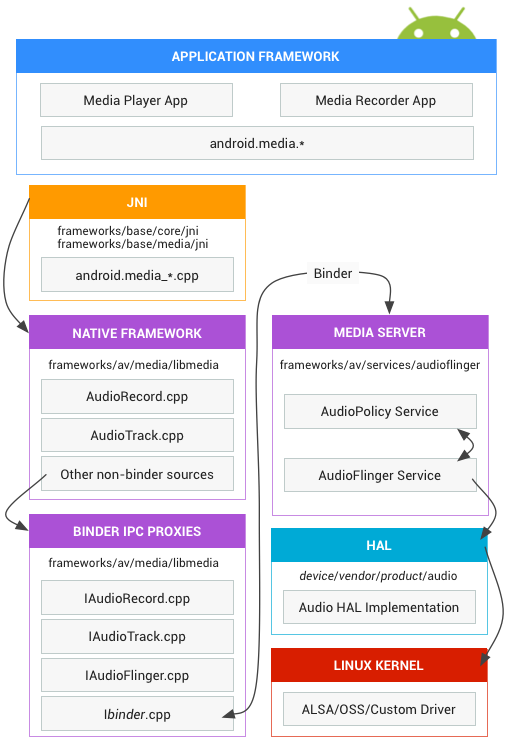
\includegraphics[width=0.5\textwidth]{img/sound_stack.png}
    \caption{The Android audio stack\cite{sound_stack}.}
    \label{fig:sound_stack}
\end{figure}

\subsection{Summary}
The sound stack on Android have several layers, which sound have to go through.
Some of these layers are more relevant for this project than others,
especially the application framework, native framework, media server and Linux kernel.
These layers should be considered when an app to solve the problem statement is designed.


